\documentclass[12pt,a4paper]{article}
\usepackage{hyperref}
\usepackage{url}
\usepackage{amsmath}
\usepackage{apacite}
\usepackage[german]{babel}
\usepackage[utf8]{inputenc}
\usepackage{graphicx}
\usepackage[T1]{fontenc}

\author{Felix Baumann, Ravinder Sangar, Jonas Winkler}
\title{Biometric Crypto-Systems}

\begin{document}

\maketitle
\tableofcontents

\section{Einleitung}
\subsection{Was sind biometrische Kryptosysteme und wozu sind sie wichtig?}
Biometrische Daten sind biologische Messwerte bzw. physische Merkmale, die zur Identifizierung von Personen dienen. Typische Beispiele sind Fingerabdruckscan, Gesichtserkennung, Iriscan und Stimmerkennung. Aber mittlerweile sollen auch die Form des Ohres, die Art, wie jemand sitzt und geht, Körpergerüche, Venenmuster auf der Hand oder Gesichtszüge eindeutig zuweisbare Merkmale sein. 
Da diese biometrischen Merkmale unveränderlich und individuell sind, werden sie dazu eingesetzt, Passwörter für elektronische Geräte, bzw. auch Schlüssel für Räume und Gebäude zu ersetzen oder zumindest zu unterstützen. \newline
Biometrische Kryptosysteme verbinden also Kryptographie und Biometrie, um von den Vorteilen aus beiden Bereich zu profitieren. Sie sichern einen kryptographischen Schlüssel mit solchen biometrischen Merkmalen oder generieren sogar aus einem biometrischen Merkmal einen kryptographischen Schlüssel. Diese Systeme ermöglichen eine sichere Authentifizierung und Schlüsselhinterlegung, ohne dass die für die Verifikation gespeicherten Informationen die biometrischen Daten der Benutzer preisgeben. \newline
Bei Biometrischen Daten wird genauso wie bei passwortbasierter Authentifizierung eine One-Way-Hashfunktion verwendet, um die Passwörter zu speichern, doch im Gegensatz zu Passwörtern, sind die biometrischen Daten nicht exakt und gleich, sondern leicht unterschiedlich und würde die Hashfunktion eine komplett andere Ausgabe geben. Die Lösung dafür sind Biometrische Kryptosysteme: Diese verwenden einen sogenannten fehlerkorrigierenden Code, der für die Erkennung und Korrektur von Fehlern zuständig, also veranlasst er, dass die Authentifizierung auch trotz variablen Faktoren, wie Licht, Entfernung, Verschmutzung etc. korrekt funktioniert. \newline
Alle wichtigen biometrischen Kryptosysteme funktionieren dabei ähnlich: 
Es wird bei der Registrierung (Enrolment) ein zufälliger Wert s gewählt. Dieser Wert wird über einen fehlerkorrigierenden Code mit dem Merkmalsdatensatz (Template) $f$ zu einem Wert $y$ verknüpft wird. Der Wert $y$ und der Hash $h(s)$ werden für die Verifikation gespeichert.
\cite{repetico}
\newline \newline
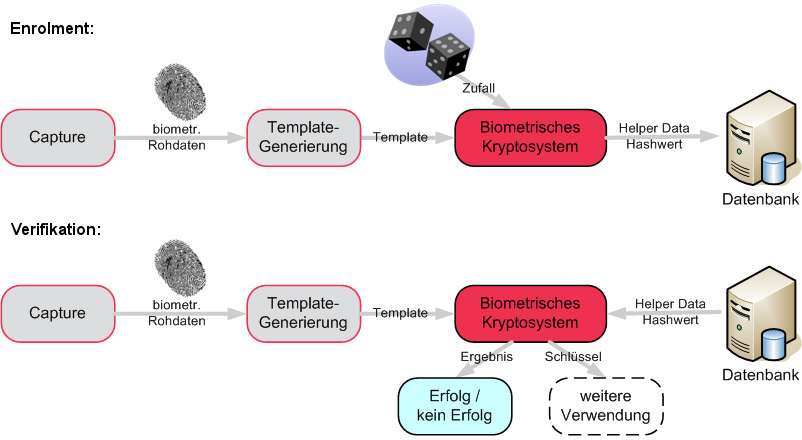
\includegraphics[scale=0.6]{08-6-052-1.jpg}
\newline
Bild: \url{http://2014.kes.info/archiv/online/images/08-6-052-1-400.jpg}

\section{Ursprung}
\subsection{Idee hinter Biometrie}
ie vermeintlich erste Nutzung von Biometrie ist die des Fingerabdrucks. Doch gibt es keine klaren Daten, wann bzw. wer den Gebrauch von Fingerabdrücken als erster genutzt hat. Jedenfalls fand man erste Spuren von Biometrie in Mesopotamien (heutige Irak), wo vor 4000 Jahren babylonische Töpfer ihre Werke mit ihren Fingerabdrücken unterschrieben. Auch für Transaktionenbestätigungen wurde mit Fingerabdrücken gearbeitet: Der Töpfer selbst hat seinen Fingerabdruck an die eine Seite des zum Beispiel Topfes angebracht und der Käufer an der anderen Seite. So wurde der Vertrag gültig gemacht und vor Fälschungen geschützt. \newline
1880 bekam der Fingerabdruck eine viel wichtigere Bedeutung, als ein bekannter Mediziner, Henry Faulds, bekannt gab, dass er jahrelang diese Biometrie untersucht habe und herausfand, dass jeder Fingerabdruck individuell und einzigartig ist und er selbst dies schon eingesetzt habe, um Betrug zu vermeiden. Schließlich schlug er vor, dass diese Erkenntnis an Tatorten eingesetzt werden soll, um Täter zu identifizieren. Natürlich war der Vorschlag von Faulds damals nicht so einfach umzusetzen, weil die nötige Technik fehlte und so wurde Faulds Erkenntnis zu seiner Zeit abgelehnt. Aber wie wir heute sehen werden Fingerabdrücke heutzutage in der Forensik genutzt.
\cite{online_signatures}
\subsection{Heutige Verwendung}
In heutiger Zeit werden auch schon andere biometrische Daten für zahlreiche Bereiche im Alltag genutzt, wie zum Beispiel Gesichtserkennung, welches mittlerweile für einigen Smartphones zur Entsperrung dient. Türschlösser werden ebenso durch einen Fingerabdruckscan ersetzt. Für Nutzer vereinfacht Biometrie so natürlich den Alltag und spart Zeit: Die Passwörter müssen nicht mehr gemerkt und eingegeben werden. 
Die Gesichtserkennung wird mittlerweile auch schon bei vielen Flughäfen eingesetzt um gesuchte Kriminelle zu erkennen. \newline
Seit 2004 in der EU und mittlerweile weltweit werden sogenannte biometrische Pässe (auch ePass) ausgegeben. Dieser enthält biometrische Daten, um die Identität eines Reisenden sicherer und schneller feststellen zu können. In diesem ePass sollen zwei biometrische Merkmale integriert sein: Zum einen ein Bild des Gesichts und zum anderen zwei Fingerabdruckbilder. Jeder biometrische Pass hat ein bestimmtes Zeichen auf der Abdeckung.
\cite{reisepass} \newline
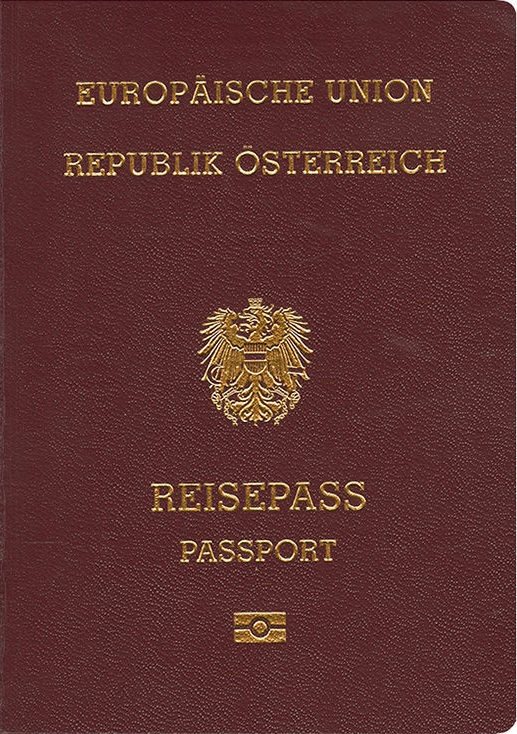
\includegraphics[scale=0.25]{Reisepass_at.jpg}
\newline
Bild: \url{https://upload.wikimedia.org/wikipedia/commons/3/3b/Reisepass_at.jpg}

\section{Problematik}
\subsection{Gefahr vor Hackangriffen}
Alle Daten, die gesammelt werden, können gehackt werden, je wichtiger der Anwendungsbereich ist, desto sicherer ist die Verschlüsselung. Da man aber heutzutage vermehrt Biometrische Daten verwendet werden, kann es dazu kommen, das andere Systeme die Daten nicht so sicher verschlüsseln und diese Daten dadurch leichter zugänglich werden.
\subsection{Biometrische Daten sind nicht veränderbar}
Wenn Passwörter geklaut werden kann man durch ändern des Passworts vielleicht noch den Schaden in Grenzen halten, wobei bei biometrischen Daten dies nicht der fall ist. Sie können nicht verändert werden und sollte jemand an diese Daten kommen, kann sehr viel Schaden dadurch entstehen, wo man keine Kontrolle mehr hat.
\cite{kaspersky}
\subsection{Duplikation von biometrischen Daten}
Ein Angreifer könnte aus der Ferne hochauflösende Fotos von Körperteilen wie Ohren aufnehmen, oder Fingerabdrucke von einem Glas kopieren, die in einem Café hinterlassen wurden. Mit diesen Informationen könnte man z.B. die Biometrischen Entsperrung von Smartphones oder anderen Geräten zu umgehen. Gegen solche Angreifer können auch biometrische Kryptosystem nicht helfen. Wobei können diese System gegen Angreifer schützen, die versuchen das Template allein aus den hinterlegten Verlgeichdaten zu ermittlen.
\cite{norton}
\section{Biometric Template Protection}
Biometric Template Protection bezeichnet ein Verfahren der biometrischen Personenerkennung. Im Gegensatz zu herkömmlichen biometrischen Erkennungsverfahren, werden jedoch hierbei die zu Beginn vom Nutzer bereitgestellten biometrischen „Infos“ (Templates) nicht als Referenzdaten gespeichert. Stattdessen werden die Referenzdaten in sogenannte \textit{Protected Templates} umgewandelt, welche dann zwar zur Authentifizierung ausreichen, aber keine Rekonstruktion der tatsächlichen Daten zulassen. Dies ist deshalb wichtig, da Fingerabdrücke, Iris-Scans, ... im Gegensatz zu Passwörtern o.Ä. nicht geändert werden können. Würde man also einmal ein Template erschleichen, so könnte man alle mit diesem Template gesicherten Geräte entsperren.

\cite{biometrictemplate_intro}
\subsection{Fuzzy Commitment}
Fuzzy Commitment beschreibt ein kryptographisches Verfahren, das die entstehenden Unschärfen, welche bei der Verwendung von biometrischen Erkennungsverfahren auftreten, berücksichtigt und dennoch die Authentifizierung ermöglicht.
\subsubsection{Commitment schemes im Allgemeinen} 
Ein kryptographisches Commitment-Schema hat folgende Funktion $G : C\times X \rightarrow W$. Um einen Wert $c\in C$ zu verschlüsseln, wird also ein „Zeuge“ $x\in X$ gewählt (normalerweise zufällig), um daraus $w = G(c,x)$ zu berechnen. Dieser Output $w$ wird oft als „blob“ oder „Safe“ bezeichnet, denn dieser kann an den Empfänger sorgenfrei übergeben werden, ohne passendem Schlüssel (Template) kann er $c$ nämlich nicht erfahren. Die Inversfunktion lautet wie oben schon kurz angeschnitten $G^{-1} : Y\times X \rightarrow C$. \\
Ein korrektes Commitment-Schema hat zwei besondere Eigenschaften: Zum ersten die Verbindlichkeit, dass es quasi nicht möglich ist, den Schlüssel $c$ zu erraten (\textit{binding}). Die zweite Eigenschaft \textit{hiding} verbietet, den Schlüssel freizugeben, sofern der Zeuge $x$ bzw. $x'$ nicht richtig ist. \\
Bei der folgenden Erklärung von Fuzzy Commitment wird ist die zu verschlüssende Nachricht $c$ der Schlüssel selbst, der Zeuge ist in unserem Fall kein Zufallswert, sondern das Template selbst.
\subsubsection{Funktionsweise}
Es gibt zwei Phasen, in die Fuzzy Commitment (oder auch andere biometrische Verschlüsselungsverfahren) eingeteilt werden: 
\begin{itemize}
\item \textit{Enrollment} - die Initialisierungsphase, das Anlegen des Templates vom User und dessen Verarbeitung
\item \textit{Authentication} - Einlesen des bereitgestellten Templates und Authentifizierung
\end{itemize}
Beim Enrollment verwendet das Verfahren einen Schlüssel, also einen zufälligen Bitstring $s$, der gemeinsam mit dem gegebnen \textit{Template} (Fingerabdruck, Iris-Scan, Gesichts-Scan) - ebenfalls als Bitstring - zur Verschlüsselung benötigt wird.
Am effektivsten funktioniert es, wenn die Bits von $s$ gleichverteilt sind, (d.h. die Wahrscheinlichkeit, dass „0“ oder „1“ auftritt, ist gleich hoch - außerdem sind die Bits voneinander unabhängig). \\
Über diesen Schlüssel $s$ wird eine One-way-Hashfunktion $h(s)$ gelegt und gespeichert. Hierbei ist wichtig, dass sie one-way ist, ansonsten wäre die Sicherheit stark gefährdet, da man $s$ berechnen könnte.
Um den anfangs erwähnten Unschärfen aufgrund von Anpressdruck, anderen Lichtverhältnissen etc. entgegenzuwirken, wird im Folgenden $s$ in einen Hamming-Code $c$ umgewandelt. Wenn $s$ eine Länge von $n$ Bits hat, so hat $c$ eine Länge von $k$ Bits mit $k > n$. Der Hamming-Code funktioniert wie folgt: An jede Stelle, die eine Potenz von 2 ist, wird ein Paritätsbit eingefügt. (Im Falle $n = 8 Bits$ bräuchte man also vier Paritätsbits an den Stellen 1, 2, 4 und 8, woraus sich Codewort mit der Länge $n + 4 = k = 12 Bits$ ergibt.) \\
Im Anschluss werden die \textbf{Stellen} derjenigen Datenbits, die den Wert 1 haben, miteinander verxort. Als Ergebnis erhält man den Bitstring, der einem den Wert der Paritätsbits - von MSB in Richtung LSB - verrät. Diese Werte werden nun eingetragen, womit das Codewort $c$ fertig ist. (Siehe Beispiel in den Slides) \\
Nun wird das biometrische Template - der Fingerabdruck, Gesichts-Scan, etc. - als $x$ mit dem Codewort $c$ verxort, und das Ergebnis als $w$ gespeichert. ($w = c \oplus x$) Es befinden sich folglich nur $w$ und $h(s)$ im Speicher und weder $x$ noch $c$ kann herausgefunden werden. \\

Wenn nun der Nutzer seinen Finger auf den Fingerabdrucksensor legt, wird Phase 2 - Authentication - aufgerufen. $w$ wird aus dem Speicher geholt und mit dem Template $x$ (Fingerabdruck) verxort, was das Kandidatenwort $c' = w \oplus x'$ liefert. Dieses wird nun mit der Umkehrfunktion des Hamming-Codes wieder entschlüsselt (i.e. auf Fehler überprüft und gegebenfenfalls korrigiert) und die Paritätsbits vom Kandidaten-Codewort $c'$ abgezogen, um einen Kandidatenschlüssel $s'$ zu erhalten. Nun wird überprüft ob die Hashfunktion $h(s)$ das gleiche Ergebnis liefert wie durch einsetzen von $h(s')$. Wenn ja, war die Authentifizierung erfolgreich. \\

Bei dem gegebenen Commitment $w = G(c,x)$ erlaubt die Wiederherstellung der ursprünglichen Nachricht $c$ mithilfe jener $x'$-Werte nahe $x$, aber nicht gezwungenerweise gleich $x$. Wie weit die $x'$-Werte von den $x$-Werten abweichen dürfen, wird von der Hamming-Distanz gemessen.  $Hd(x) = |x - x'|$. Diese darf beim Hamming-Code nicht mehr als 3 betragen, um nicht von der Authentifizierung ausgeschlossen zu werden. Eine weitere Eigenart von Fuzzy Commitment ist, dass seine Sicherheit stark von der Wahl des zufälligen Wertes $c\in C$ abhängig ist. Die \textit{hiding}-Eigenschaft von fuzzy commitment bedeutet, dass der Blob $w$ nur einen sehr kleinen Teil des $c$-Wertes wiederherstellen kann, wordurch es mit den richtigen Parametern möglich ist, $w$ „öffentlich“ zu machen, da es nicht möglich ist, $c$ vollständig zu erfahren.

\cite{fuzzy_commitment} 
\newline
In Betrachtung des folgenden Bildes lässt sich die Funktionsweise von Fuzzy Commitment folgenderweise zusammenfassen: Während dem Enrolment-Prozess (Verarbeitung des Templates), wird eine zufällige Zahl $S$, und deren Hashfunktion $h(S)$ generiert. $S$ wird dann als Hammingcode vom Encoder $ENC$ zu dem Codewort $C$ weiterverarbeitet. Das binär verarbeitete Template $x$ wird mit $c$ kombiniert, und als $W = X \oplus C$ gespeichert. Zur Authentifizierung wird eine neue biometrische Datei eingelesen und daraus ein neues Template $Y$ generiert. Mit $W$ kombiniert, ergibt es ein Kandidaten-Codewort $C' = W \oplus Y = C \oplus (X \oplus Y)$. $C'$ wird in einen Hamming-Decoder $DEC$ geworfen, um den Kandidatenschlüssel $S'$ zu erhalten. Wenn nun $h(S) = h(S')$, so ist der erhaltene Schlüssel korrekt, und $X$ und $Y$ haben identische Eigenschaften. \\
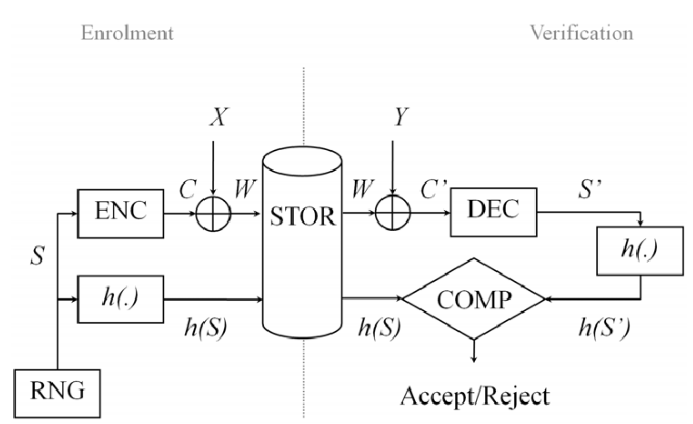
\includegraphics[scale=0.45]{fcs.png} \\
Bild: \url{https://www.cosy.sbg.ac.at/~uhl/biometrics_slides.pdf} - Seite 67
\subsubsection{Vorteile}
Gerade für das Verwenden von biometrischen Daten zum Entsperren von Sicherheitssystemen, bietet das fuzzy commitment die nötige Unschärfe, die nicht immer vorhandene Beständigkeit von Fingerabdrücken (Fettfinger, Winkel) oder Gesichtern (Verschlafenheit, Lichtverhältnisse), trotzdem zu entschlüsseln. Außerdem werden die Templates nicht direkt gespeichert, weshalb im Falle eines Hackangriffes die Biometrics des Nutzers geschützt wären.
\subsubsection{Nachteile}
Als Nachteil könnte man dem Fuzzy Commitment minimal weniger Sicherheit gegenüber anderen Commitments, die den exakten Schlüssel zum Wiederherstellen des originalen Inputs benötigen, rezitieren. Bei der Verschlüsselung mit biometrischen Daten ist die Verwendung von 100\% akkuraten Schlüsselwerten jedoch völlig unrealistisch. Außerdem muss die Länge des Schlüssels derjenigen des biometrischen Templates entsprechen, da dies Voraussetzung für die XOR-Operation ist.

\subsection{Fuzzy Vault}
Das Fuzzy vault scheme ist ein Algorithmus, der zur Sicherung von biometrischen Templates verwendet wird.
\subsubsection{Funktionsweise}
Im Folgenden wird die Funktionsweise anhand des gewählten Beispiels von Ari Juels erklärt: Alice möchte jemanden finden, der dieselben Interessen wie sie hat, aber sie möchte diese Interessen nicht freigeben. Daher veröffentlicht sie eine Menge der Interessen, welche jedoch verschlüsselt sind. Wenn jetzt Bob ähnliche Interessen wie Alice hat, kann er diese Menge anhand seiner eigenen Interessen entschlüsseln und die Nachricht lesen. Wenn Bob nicht dieselben Interessen hat, dann wird er nicht in der Lage sein, die Nachricht zu entschlüsseln. \newline
Mit dem fuzzy vault Konstruktionsprinzip „sperrt“ Alice ihre Nachricht $s$ in einer Menge $A$, welche den vault hervorbringt. Bob kann den vault nur dann mit seiner eigenen Menge $B$ entsperren, wenn $A$ und $B$ sich großteils überlappen, sprich $A\cap B$ ist möglichst groß. Daher kann man das fuzzy vault als fehlertolerant sehen, da sich die Mengen nicht zu 100\% übereinstimmen müssen. Der Key $s$ von Alice, welcher hier in einer Menge steckt, bleibt privat.
\newline
Die Mengen müssen nicht geordnet sein, also echte Mengen und keine Folgen von Symbole.
\newline
Diese Methode wird oft für Fingerprintverfahren verwendet. Anstelle des gesamten Fingerabdrucks werden Charakteristiken gespeichert, \textit{biometric templates} genannt.
Die Fingerprintscanner werden oft beim Scannen desselben Fingers ein Template $A'$ erstellen, welches zwar ähnlich, aber nicht gleich dem Template $A$ ist. Die Sensoren sind also fehleranfällig und oft nicht in der lage, das gescannte Template zu 100\% zu reproduzieren. Daher sichert Alice im vault einen PIN, welcher den Fingerabdruck beschreibt.
\subsubsection{LOCK-Algorithmus}
Wir verwenden einen Reed-Solomon-Decode Algorithmus, kurz $RS_{DECODE}$, welcher ermittelt, ob sich mindestens $\frac{k+t}{2}$ Punkte einer Menge mit einer gemeinsamen polynomiell berechenbaren Funktion beschreiben lassen. Der zu verschlüsselnde Key $s$ wird als RS-Codewort dargestellt. Im Anschluss werden die Punkte $(x_{i}, y_{i})$ berechnet, wobei der $x$ Wert die Werte $a_{i} \in A$ repräsentiert. Der Körper $F$ 
\newline
\hspace*{10mm}$ X,R\rightarrow \emptyset$ \newline
\hspace*{10mm}$s \rightarrow p$\newline
\hspace*{10mm}$for \; i=1 \; to \; t $\newline
\hspace*{15mm}$(a_{i}, p(a_{i})) \rightarrow (x_{i}, y_{i})$\newline
\hspace*{15mm}$X\bigcup \{x_{i}\} \rightarrow X$\newline
\hspace*{15mm}$R\bigcup \{(x_{i},y_{i})\} \rightarrow R$\newline
\hspace*{10mm}$for \; i=t+1 \; to \; r$\newline
\hspace*{15mm}$x_{i} \in F - X$\newline
\hspace*{15mm}$y_{i} \in F - \{ (x_{i},y_{i} \}$\newline
\hspace*{15mm}$R\cup \{(x_{i},y_{i})\} \rightarrow R$\newline
\hspace*{10mm}$return\;R$\newline
\newline
Die Ausgabe $R$ ist nicht geordnet nach $x_i$, damit keine Informationen über dem Auswahlverfahren geleakt werden. Die Ausgabe $R$ repräsentiert den fuzzy vault $V_{A}$. Diese Menge ist eine Kombination der Informationen des Fingerabdrucks, sowie den $chaff$-points. $Chaff$-points sind zufällig generierte $(x_{i},y_{i})$ Paare $\in$ $F$, die denen von $A$ und $p(A)$ ähneln. Sie werden verwendet um die resultierende Menge zu manipulieren, damit auch wenn die Menge abgefangen wird, man nicht direkt zu den Daten gelangt. Durch den $chaff$-points erhält man also eine Menge welche mit „Fehlern“ behaftet ist. Wie bereits beschrieben kann man den Key nur mit einer zweiten Menge B entschlüsseln, welche nicht zu sehr von A abweicht. Hat der Angreifer also kein Template welches zu A passt, wird er nicht in der Lage sein die tatsächlichen Punkte des Fingerabdrucks von den $chaff$-points zu unterscheiden. 
\subsubsection{UNLOCK-Algorithmus}
\hspace*{10mm}$ Q \rightarrow \emptyset$ \newline
\hspace*{10mm}$for \; i=1 \; to \; t $\newline
\hspace*{15mm}$R \xrightarrow{\text{ $b_{i}, \circ $}} (x_{i}, y_{i})$\newline
\hspace*{15mm}$Q\bigcup (x_{i},y_{i}) \rightarrow Q$\newline
\hspace*{10mm}$RS_{DECODE}(k,Q) \rightarrow s'$\newline
\hspace*{10mm}$return\; s' $\newline
\newline
Damit der Vault „geöffnet“ werden kann, wird eine Menge $B$ benötigt, die der Menge $A$ ähnelt. Wichitg ist hier, dass $b_{i} \in B \in F$ zutrifft. Denn wendet man nun die Verknüpfung $\circ$ auf $b_{i}$ an, erhält man den dazugehörigen Polynomialwert und bildet somit den Punkt $(x_{i},y)$, ist dieser Punkt $\in$ R, erreichen wir die Gleichheit $(b_{i},y) = (x_{i},y_{i})$. Ist die Gleichheit nicht gegeben weisen wir dem wert $(x_{i},y_{i})$ $null$ zu. Ist $B$ so eine Menge, dann werden durch $B$ die korrekten Punkte gefunden. Die restlichen Punkte sind also die $chaff$-points und somit auch der Unterschied zwischen $A$ und $B$. Diese Punkte werden mithilfe vom $RS_{DECODE}$-Algorithmus gefiltert. Auch hier ist der springende Punkt, dass $RS_{DECODE}$ nur dann die Menge erfolgreich filtert, wenn d Ist dies erfolgreich, erhalten wir dadurch ein $s'$, wleches gleich wie $s$ ist. Ist $s' = null$, dann ist der Schnitt der zwei Mengen zu klein.

\cite{michigan}
\subsubsection{Vorteile}
Die Konstellation des $fuzzy$-$vaults$ ist gerade für Fingerabdrucksensoren sehr praktisch, da die Sensoren bzw. der Fingerabdruck selbst "Fehler" verursachen, und das ausnutzen des 
Die Sicherheit ist stark von den Chaff-points abhängig, denn dadurch wird es schwieriger, die „korrekten“ Punkte von den Chaff-points zu unterscheiden. Die Länge des Schlüssels $s$ spielt dabei keine Rolle, da die Punkte relevant sind.
\subsubsection{Nachteile}
Das $fuzzy$-$vault$-scheme ist im Gegensatz zu anderen Verschlüsselungsverfahren nicht sehr sicher bzw die Sicherheit hängt völlig von der größe der Mengen, die zum erzeugen des $vaults$ verwendet werden, und dessen Berechnungen ab.  
\bibliographystyle{apacite}
\bibliography{source}
\end{document}

